\chapter{Introduction}\label{ch:introduction}
In this chapter, the project is introduced and motivated. Furthermore, a brief description is presented for stereo vision and the use for it at HSA systems. Lastly, this chapter also describes a delimitation of the project and report.\\

\section{Introduction to stereo vision}\label{sec:stereo vision}
In 280 A.D the greek mathematician Euclid discoverd that the perception of depth is caused by each eye receiving a dissimilar image of the same object. Throughout history different people have been working on this concept. In 1933 Sir Charles Wheatstone began to mimic depth perception and forced the perception of depth by developing the stereoscope. The stereoscope uses images taken by two cameras placed next to each other and the stereoscope then isolates the images so each eye only sees one image. This mimics depth perception and the viewer would precieve depth in the images. \cite{lit:historyofstereophoto}\\

Around 1970 computer vision began appearing and a big part of this area is stereo vision: the measurement of depth mimicing the human vision using two cameras \cite{Szeliski2010}. The ability to measure depth enables a computer to distinguish between objects and hence better interact with and react on the world.\\

\section{HSA systems}
\begin{figure}[ht!]
  \centering
  \begin{subfigure}[t]{0.45\textwidth}
    \centering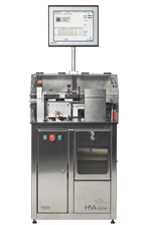
\includegraphics[height=5cm]{figures/pv650_225px}
    \caption{PV650C\cite{HSAsystems}}
    \label{fig:pv650c}
  \end{subfigure}\hspace{0.5cm}
  \begin{subfigure}[t]{0.45\textwidth}
    \centering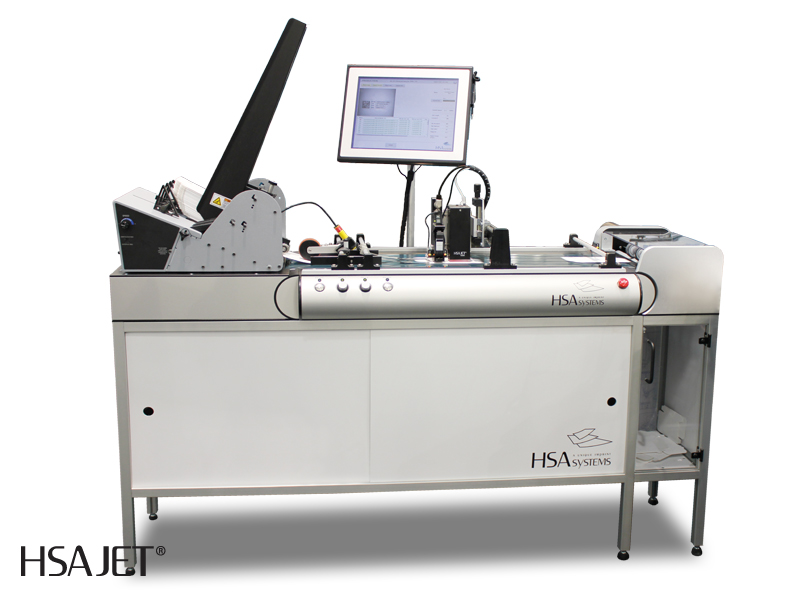
\includegraphics[height=5cm]{figures/layflat1_big}
    \caption{Pharma lay-flat media \cite{HSAsystems}\label{fig:layflat}}
  \end{subfigure}
  \caption{Some of HSA systems products\label{fig:hsasproducts}}
\end{figure}
HSA systems is a danish company which develops and manufactures high-resolution inkjet printer systems and a range of other products. Figure \vref{fig:hsasproducts} shows some of these printer systems. These systems prints labels, bar codes etc on packages and verify the quality print.\\

HSA systems wishes to track packages going through their printer systems. A strategically placed stereo vision camera will enable them to know how many and where these packages are in the printer system. In case of errors and the like the printer system is then able to notice when the conveyor belt in their system is empty and ready to reset.\\

In future uses, HSA systems would like the stereo vision system to have very precise depth measurements of \SI{\leq 2}{\milli\meter} at distances between 0.5-1.5 m.

\section{Motivation}\label{sec:intromotiv}
The area of stereo vision has been researched thoroughly and precise algorithms have been found but most algorithms are very heavy computational wise. HSA systems wishes for a stereo vision system which can run real-time (10 fps) and have a high precision of \SI{\leq 2}{\milli\meter} between 0.5 m and 1.5 m.

\section{Problem description}
HSA systems wishes to track packages going through their system. A strategically placed stereo vision camera will enable them to know how many and where these objects are in the system. \\
The following questions will be researched:
\begin{itemize}
  \item What obstacles occur within stereo vision
  \item Which stereo algorithms exist which are efficient while having good results
  \item How can an architecture be design and optimized for executing a stereo vision algorithm
\end{itemize}

\section{Delimitation}
This project is mainly concerned with the design and implementation of a hardware design for a FPGA. This project will not focus on developing a new stereo vision algorithm. Limitations and issues with stereo vision algorithms will be analyzed but simpler solution will be used for most obstacles.

\section{Report Structure and Design Process}\label{sec:a3model}
The A$^3$ model is a basic design model used internally at AAU and is illustrated on figure \vref{fig:A3model}. The model consists of three design domains which can be explored and the report is structured after this model. These domains are Application, Algorithm and Architecture.\\
\begin{figure}[ht!]
  \centering
  \includegraphics[scale=0.25]{figures/A3model.jpg}
  \caption{A$^3$ model}
  \label{fig:A3model}
\end{figure}

The search for a solution starts in the application domain where the problem and application is being explored. Chapter \vref{ch:appanalysis}: Application Analysis will explore the Application domain and the resulting specification for the application are presented in chapter \vref{ch:req}. The problem and application - which has been specified by HSA systems - is specified in this chapter and will be explored further in chapter \vref{ch:appanalysis}.\\~\\
As represented by the solid arrows on figure \vref{fig:A3model}, there are several possible algorithms that may match a specified application, and several architectures that may be used to implement a given algorithm. Exploration of the algorithm is described in chapter \vref{ch:alganalysis} .\\~\\
Chapter \vref{ch:designmet} will describe a methodology to traverse from an algorithm in the algorithm domain to some hardware architecture in the architecture domain.\\~\\
Notice the dashed arrows in figure \vref{fig:A3model}. These arrows show that when exploring one domain new information might arise which calls for changes in a former domain, and requiring a new iteration through the domains.\\~\\

Chapter \vref{ch:acctest} specifies the testing done to determine whether the found solution complies with the requirements in chapter \vref{ch:req}. Chapter \vref{ch:conclusion} concludes the project and its findings. 


